\section{Монгол улсын хүн ам, дундаж цалин, ДНБ-г ашигласан дашбоард}

Энэхүү дашбоардыг дадлагын төлөвлөгөөний суралцах эхний 4-н долоо хоногт долоо долоон хоногоор суралцсан зүйлсээ ашиглан сайжруулан хийсэн.

Сурах ур чадвар: 
\begin{itemize}
    \item Tableau-ийн анхан болон ахисан түвшиний зүйлсийг суралцах
    \item Дашбоард өрөхөд шаардлагатай чадваруудыг суралцах
\end{itemize}

\subsection{Сурах үйл явцын хийсэн дашбоард}

Дашбоардыг хийхдээ анхандаа өгөгдлөө бэлдэх буюу 1212.mn-ээс нээлттэй Монгол улсын хүн амын тоо, дундаж цалингийн тоон мэдээлэл, ДНБ-ы хэмжээ зэргийн статистик мэдээллийг хүснэгт хэлбэрээр аван өгөгдлөө цэвэрлэх, зөв бүтэцтэй болгон засварчилсан. Түүний дараа алхам алхамуудаар table-ийн ойлголт, хэрэглүүрүүдийг суралцан дашбоардаа хийгдсэн.

Дашбоард: \url{https://public.tableau.com/app/profile/adiya.hella/viz/_16880920782180/Story1}
\begin{figure}
	\centering
	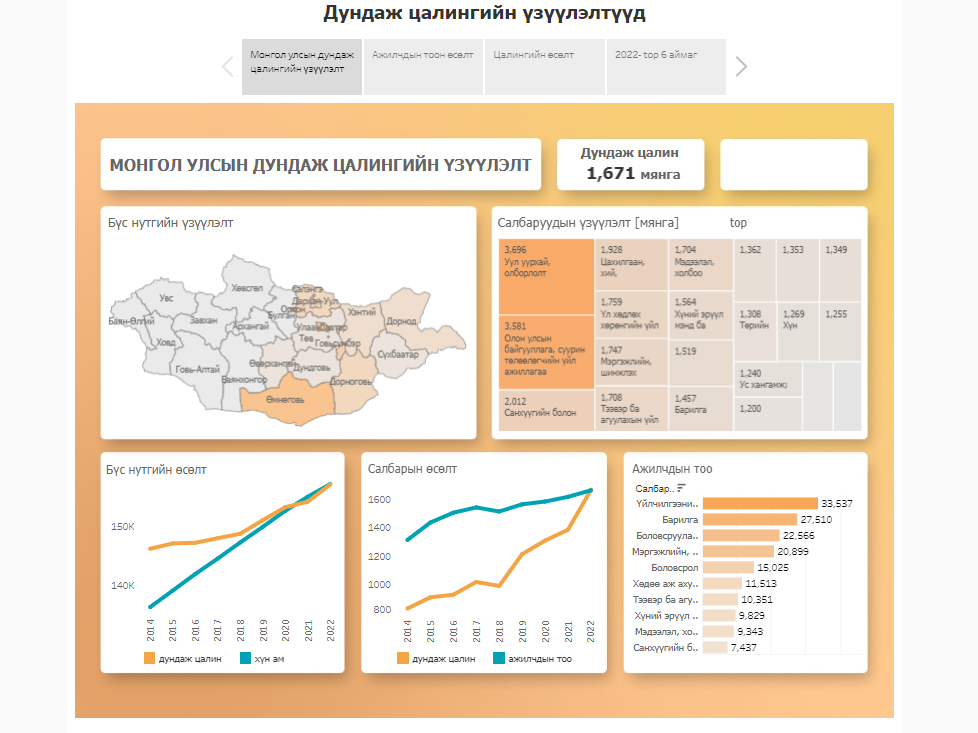
\includegraphics[width=15cm]{images/dash1.PNG}
	\caption{Суралцах явцын дашбоард}
	\label{fig:form}
\end{figure}


\subsection{Төслийн багт оролцон гүйцэтгэсэн ажил}

Энэхүү дашбоардыг өмнө хийсэн байсан дашбоард нь хэрэглэгч буюу захиалагчийн үнэлэмжинд хүрээгүй тул хамт дадлагын хөтөлбөрт хамрагдсан оюутантай хамтран эхнээс нь хэрэглэгчийн шаардлагад нийцүүлэн гүйцэтгэсэн.


Дашбоард: \url{https://public.tableau.com/app/profile/adiya.hella/viz/13x7/1366x768}
\begin{figure}
	\centering
	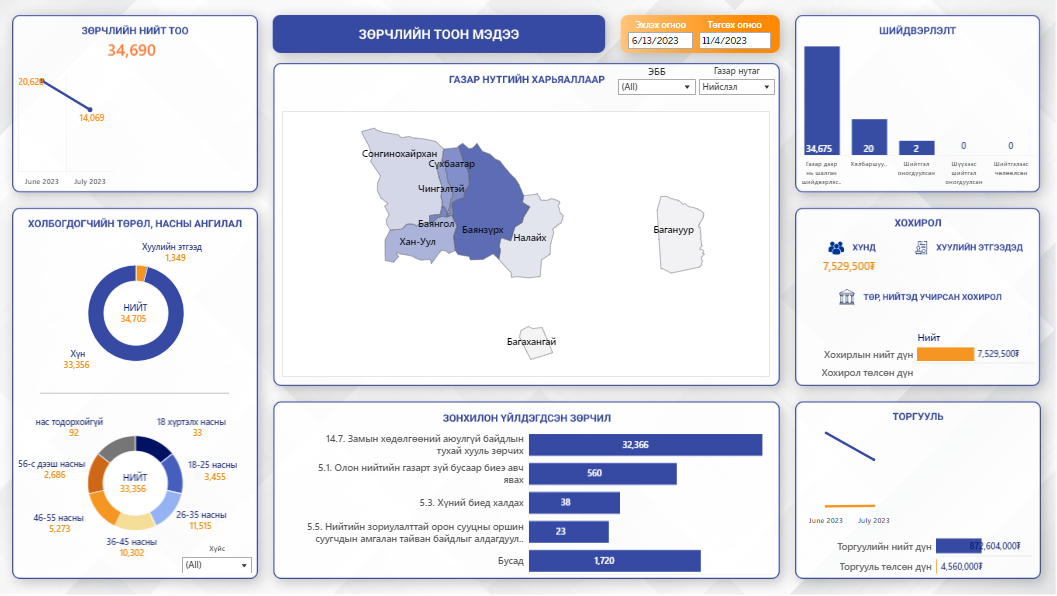
\includegraphics[width=15cm]{images/dash2.PNG}
	\caption{Төслийн явцын дашбоард}
	\label{fig:form}
\end{figure}
